\documentclass[fleqn, table, 10pt]{beamer}

\usepackage{comment}
\usepackage{booktabs}
\usepackage{threeparttable}
\usepackage{setspace}
\usepackage{hyperref}
\usepackage{import}
\usepackage{tikz}
\usepackage{caption}
\usepackage{amsmath}
\usepackage{verbatim}
\usepackage{fancyvrb}

%\def\verbatim@font{\footnotesize\ttfamily}

\usetheme{AnnArbor}

\title[Exporting Stata Tables and Figures to \LaTeX{}]{\textbf{Exporting Stata Tables and Figures to \LaTeX{}}}
\date[July 2, 2013]{July 2, 2013}
\author[J. Fogel]{Jamie Fogel}

\def\results{S:/trainings/exporting_stata_tables_figures/results}


\begin{document}


\begin{frame}[plain]
    \titlepage
\end{frame}

\begin{frame}{Why create figures and tables using Stata and \LaTeX{}?}
    \begin{itemize}
        \item Robustness --- By automating everything you reduce the likelihood of making an error such as mislabeling figures or inputting elements of a table incorrectly.
        \item Repeatability and editability --- You will have code for the entire process of creating your figure/table so it is simple to recreate your figures/tables, make minor edits to them, or create additional versions with subtle differences.
        \item Appearance --- The combination of Stata and \LaTeX{} can produce tables and figures that are far more visually appealing than anything you will create in Word or Excel.
        \item Ease of updating --- Suppose you want to add additional years of data to your regression or realize that you made a mistake in creating your data set. Updating your tables is as simple as re-running your Stata code and re-compiling your \LaTeX{} document.
    \end{itemize}
\end{frame}

\begin{frame}{Which looks better?}
    \begin{columns}[T]
        \column{.45\linewidth}
            \begin{table}
                \caption{Ugly Excel Table}
                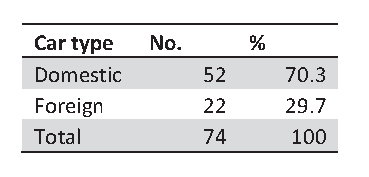
\includegraphics{\results/ugly_excel_table.eps}
            \end{table}
        \column{.45\linewidth}
            \begin{table}
            \caption{Pretty \LaTeX{} Table}
            \label{mytablelabel}
            \begin{tabular}{lrr}
                Car type&No.&\% \\
                \midrule
                Domestic&52.0&70.3 \\
                Foreign&22.0&29.7 \\
                Total&74.0&100.0 \\
            \end{tabular}
            \end{table}
    \end{columns}
\end{frame}

\begin{frame}{What I will cover today}
    \begin{enumerate}
        \item \textbf{tabout} --- Outputting tabulations of variables
        \item \textbf{esttab/estout} --- Outputting regression output and other statistical tables
        \item \textbf{graph export} --- Export Stata figures
    \end{enumerate}
\end{frame}

\section{tabout}

\begin{frame}[fragile]{What is \textbf{tabout}?}
     \textbf{tabout} allows the user to produce oneway or twoway tables of frequencies and/or percentages, as well as tables of summary statistics. These tables can be exported in a number of different formats, including .scv, but the most useful is .tex, which is used by \LaTeX{}. A much more thorough treatment of \textbf{tabout} can be found at \url{http://www.ianwatson.com.au/stata/tabout_tutorial.pdf}.
\end{frame}

\begin{frame}[fragile]{A simple tabulation}
    The below command will produce a simple oneway tabulation of the variable \emph{foreign} and save it as a .tex file for use in a \LaTeX{} document: \\
    \vspace{.5cm}
    \textbf{tabout foreign using `filepath'tabout\_foreign.tex, replace style(tex)} \\ \pause
    \vspace{.5cm}
    \begin{columns}[t]
        \column{.5\textwidth}
         Code produced by \textbf{tabout} \
            \begin{verbatim}
Car type&No. \\
\hline
Domestic&52.0 \\
Foreign&22.0 \\
Total&74.0 \\
            \end{verbatim}
        \column{.5\textwidth}
            Which, when compiled, looks like \\
            \vspace{.25cm}
            \begin{tabular}{lr}
                Car type&No. \\
\hline
Domestic&52.0 \\
Foreign&22.0 \\
Total&74.0 \\

            \end{tabular}
    \end{columns}
\end{frame}

\begin{frame}[fragile]{ Now let's make the table prettier by using the ``booktabs'' option and add a column for the column percentage}
   
    \vspace{.5cm}
    \textbf{tabout foreign using `filepath'tabout\_foreign2.tex, replace style(tex) /// \\ cells(freq col) booktabs} \\
    \pause
    \begin{columns}[T]
        \column{.5\textwidth}
            \flushleft
            \begin{verbatim}
Car type&No.&\% \\
\midrule
Domestic&52.0&70.3 \\
Foreign&22.0&29.7 \\
Total&74.0&100.0 \\
            \end{verbatim}
        \column{.5\textwidth}
            \begin{tabular}{lrr}
                 Car type&No.&\% \\
\midrule
Domestic&52.0&70.3 \\
Foreign&22.0&29.7 \\
Total&74.0&100.0 \\

            \end{tabular}
    \end{columns}
\end{frame}

\begin{frame}[fragile]{We could also do a twoway cross-tab}
    \vspace{.5cm}
    \textbf{tabout foreign over40mpg using `filepath'tabout\_foreign\_over40mpg.tex, ///
        replace style(tex) cells(freq col)} \\
    \pause
    \vspace{.5cm}
    \begin{tabular}{lrrrrrr}
         & \multicolumn{6}{c}{over40mpg} \\
Car type & \multicolumn{2}{c}{0} & \multicolumn{2}{c}{1} & \multicolumn{2}{c}{Total} \\
&No.&\%&No.&\%&No.&\% \\
\hline
Domestic&52.0&71.2&0.0&0.0&52.0&70.3 \\
Foreign&21.0&28.8&1.0&100.0&22.0&29.7 \\
Total&73.0&100.0&1.0&100.0&74.0&100.0 \\

    \end{tabular}
\end{frame}

\begin{frame}[fragile]{Summary statistics for MPG and weight, broken down by foreign or domestic car}
    \vspace{.5cm}
    \textbf{tabout foreign using `filepath'tabout\_sumstats.tex, replace sum ///
        cells(mean mpg  median mpg mean weight median weight) style(tex)} \\
    \pause
    \vspace{.5cm}
    \begin{tabular}{lrrrrrr}
        Car type&Mean&Median&Mean&Median \\
&mpg&mpg&weight&weight \\
\hline
Domestic&19.8&19.0&3,317.1&3,360.0 \\
Foreign&24.8&24.5&2,315.9&2,180.0 \\
Total&21.3&20.0&3,019.5&3,190.0 \\

    \end{tabular}
\end{frame}

\begin{frame}[fragile]{So how do I actually create the table in \LaTeX{}?}
    \textbf{The ``tabular'' environment!} \\
    \begin{itemize}
        \item The \textbf{tabular} environment is opened by \verb+\begin{tabular}{specs}+ and ends with \verb+\end{tabular}+, where \emph{specs} defines how many columns the table will have and how they should be aligned.
        \item \LaTeX{}'s \textbf{tabular} environment has a number of commands that control the look of your table, but the two most important are \verb+&+ and \verb+\\+. The \verb+&+ command  delimits cells within a table and \verb+\\+ ends a line.
    \end{itemize}
    The below table, therefore, has one left-aligned column followed by two right-aligned columns: \\
    \vspace{.5cm}
    \pause
    \begin{columns}[t]
        \column{.5\textwidth}
            \vspace{-1.5cm}
            {\footnotesize
            \begin{verbatim}
\begin{tabular}{lrr}
    Car type&No.&\% \\
    \midrule
    Domestic&52.0&70.3 \\
    Foreign&22.0&29.7 \\
    Total&74.0&100.0 \\
\end{tabular}
            \end{verbatim}
            }
        \column{.5\textwidth}
            \begin{tabular}{lrr}
                 Car type&No.&\% \\
\midrule
Domestic&52.0&70.3 \\
Foreign&22.0&29.7 \\
Total&74.0&100.0 \\

            \end{tabular}
    \end{columns}
\end{frame}

\begin{frame}[fragile]{Getting a little bit fancier}
    Although the above examples all successfully produce a table in \LaTeX{}, you will usually enclose your \textbf{tabular} within a \textbf{table}. This allows you to include a caption and/or a label. This is especially useful if you would like to include a table of contents and hyperlinks.

    \begin{columns}[t]
        \column{.5\textwidth}
            {\footnotesize
            \begin{verbatim}
\begin{table}
    \caption{Origin of Cars}
    \label{mytablelabel}
    \begin{tabular}{lrr}
        Car type&No.&\% \\
        \midrule
        Domestic&52.0&70.3 \\
        Foreign&22.0&29.7 \\
        Total&74.0&100.0 \\
    \end{tabular}
    \footnotesize My footnote...
    \end{table}
            \end{verbatim}
            }
        \column{.5\textwidth}
        \begin{table}
            \caption{Origin of Cars}
            \label{mytablelabel}
            \begin{tabular}{lrr}
                 Car type&No.&\% \\
\midrule
Domestic&52.0&70.3 \\
Foreign&22.0&29.7 \\
Total&74.0&100.0 \\

            \end{tabular}\\
            \footnotesize My footnote...
        \end{table}
    \end{columns}
\end{frame}

\begin{frame}[fragile]{But didn't \textbf{tabout} create the table for me?}

\textbf{tabout} generates code for your table but does not create the opening and closing text for it (although with the right options I believe 
    it is possible to automatically generate that code as well). To include another .tex file in your document you use \LaTeX{}'s \verb+\input{}+
    command. In the above example \textbf{tabout} saved the table as ``tabout\_foreign2.tex.'' Therefore, the simplest way to create your table 
    in a \LaTeX{} document is as follows:

    \begin{columns}[t]
        \column{.5\textwidth}
            {\footnotesize
            \begin{verbatim}
\begin{table}
    \caption{Origin of Cars}
    \label{mytablelabel}
    \begin{tabular}{lrr}
        Car type&No.&\% \\
\midrule
Domestic&52.0&70.3 \\
Foreign&22.0&29.7 \\
Total&74.0&100.0 \\

    \end{tabular}\\
    \footnotesize My footnote...
\end{table}
            \end{verbatim}
            }
        \column{.5\textwidth}
        \begin{table}
            \caption{Origin of Cars}
            \label{mytablelabel}
            \begin{tabular}{lrr}
                 Car type&No.&\% \\
\midrule
Domestic&52.0&70.3 \\
Foreign&22.0&29.7 \\
Total&74.0&100.0 \\

            \end{tabular}\\
            \footnotesize My footnote...
        \end{table}
    \end{columns}
\end{frame}


\section{esttab/estout}

\begin{frame}{What are esttab and estout?}
    \footnotesize{
    The \textbf{estout} package is a user-written package which provides tools for producing publication-quality tables in Stata. It contains
    the following programs:
    \begin{itemize}
        \item esttab: Produces publication-style regression tables that display nicely in Stata's results window or, optionally, are exported to formats such as CSV, RTF, HTML, or \LaTeX{}. esttab is a user-friendly wrapper for the estout command. \pause
        \item estout: Generic program to compile a table of coefficients, "significance stars", summary statistics, standard errors, t- or z-statistics, p-values, confidence intervals, or other statistics for one or more models previously fitted and stored. The table is displayed in the results window or written to a text file. \pause
        \item eststo: Utility to store estimation results for later tabulation. eststo is an alternative to official Stata's estimates store. Main advantages of eststo over estimates store are that the user does not have to provide a name for the stored estimation set and that eststo may be used as a prefix command. \pause
        \item estadd: Program to add extra results to the returns of an estimation command. This is useful to make the the results available for tabulation. \pause
        \item estpost: Program to prepare results from commands such as summarize, tabulate, or correlate for tabulation by esttab or estout. \pause
    \end{itemize}
    }
    \footnotesize For further details see \url{http://repec.org/bocode/e/estout/index.html} or \\ \url{http://repec.org/bocode/e/estout/esttab.html}
\end{frame}

\begin{frame}{esttab}
    For the most part you will want to use \textbf{esttab} rather than \textbf{estout} because it produces nicely-formatted tables suitable
        for export as \LaTeX{}, CSV, RTF, or HTML formats. All of \textbf{estout}'s options are also available in \textbf{esttab}, however the
        reverse is not true. Additionally, \textbf{esttab} produces all of the code for opening the table and tabular environment that we had
        to provide ourselves when using tabout.
\end{frame}

\begin{frame}[fragile]{Let's produce a simple regression table using the auto data set.}
    
    \vspace{1cm}
    \begin{columns}[T]
        \column{.5\linewidth}
            \footnotesize{
            \begin{verbatim}
sysuse auto, clear
eststo clear
eststo: reg price mpg weight
eststo: reg price mpg foreign
eststo: reg price mpg weight foreign
esttab using `filepath'table1.tex, ///
    replace booktabs compress      ///
    addnote("Your footnote here")
            \end{verbatim}
            }
\pause
        \column{.5\linewidth}
            \tiny{
                {
\def\sym#1{\ifmmode^{#1}\else\(^{#1}\)\fi}
\begin{tabular}{l*{3}{c}}
\toprule
          &\multicolumn{1}{c}{(1)}&\multicolumn{1}{c}{(2)}&\multicolumn{1}{c}{(3)}\\
          &\multicolumn{1}{c}{price}&\multicolumn{1}{c}{price}&\multicolumn{1}{c}{price}\\
\midrule
mpg       &   -49.51         &   -294.2\sym{***}&    21.85         \\
          &  (-0.57)         &  (-5.28)         &   (0.29)         \\
\addlinespace
weight    &    1.747\sym{**} &                  &    3.465\sym{***}\\
          &   (2.72)         &                  &   (5.49)         \\
\addlinespace
foreign   &                  &   1767.3\sym{*}  &   3673.1\sym{***}\\
          &                  &   (2.52)         &   (5.37)         \\
\addlinespace
\_cons    &   1946.1         &  11905.4\sym{***}&  -5853.7         \\
          &   (0.54)         &  (10.28)         &  (-1.73)         \\
\midrule
\(N\)     &       74         &       74         &       74         \\
\bottomrule
\multicolumn{4}{l}{\footnotesize \textit{t} statistics in parentheses}\\
\multicolumn{4}{l}{\footnotesize Your footnote here}\\
\multicolumn{4}{l}{\footnotesize \sym{*} \(p<0.05\), \sym{**} \(p<0.01\), \sym{***} \(p<0.001\)}\\
\end{tabular}
}

            }
    \end{columns}
\end{frame}

\begin{frame}[fragile]{Alternatively, we could explicitly name each set of regression estimates and \textbf{esttab} any combination of the stored estimation sets.}
    
    \vspace{1cm}
    \begin{columns}[T]
        \column{.5\linewidth}
            \footnotesize{
            \begin{verbatim}
sysuse auto, clear
eststo clear
eststo e1: reg price mpg
eststo e2: reg price mpg weight
eststo e3: reg price mpg foreign
eststo e4: reg price mpg weight foreign
esttab e2 e3 e4                    ///
    using `filepath'table1.tex,    ///
    replace booktabs compress      ///
    addnote("Your footnote here")
            \end{verbatim}
            }
        \column{.5\linewidth}
            \tiny{
                {
\def\sym#1{\ifmmode^{#1}\else\(^{#1}\)\fi}
\begin{tabular}{l*{3}{c}}
\toprule
          &\multicolumn{1}{c}{(1)}&\multicolumn{1}{c}{(2)}&\multicolumn{1}{c}{(3)}\\
          &\multicolumn{1}{c}{price}&\multicolumn{1}{c}{price}&\multicolumn{1}{c}{price}\\
\midrule
mpg       &   -49.51         &   -294.2\sym{***}&    21.85         \\
          &  (-0.57)         &  (-5.28)         &   (0.29)         \\
\addlinespace
weight    &    1.747\sym{**} &                  &    3.465\sym{***}\\
          &   (2.72)         &                  &   (5.49)         \\
\addlinespace
foreign   &                  &   1767.3\sym{*}  &   3673.1\sym{***}\\
          &                  &   (2.52)         &   (5.37)         \\
\addlinespace
\_cons    &   1946.1         &  11905.4\sym{***}&  -5853.7         \\
          &   (0.54)         &  (10.28)         &  (-1.73)         \\
\midrule
\(N\)     &       74         &       74         &       74         \\
\bottomrule
\multicolumn{4}{l}{\footnotesize \textit{t} statistics in parentheses}\\
\multicolumn{4}{l}{\footnotesize Your footnote here}\\
\multicolumn{4}{l}{\footnotesize \sym{*} \(p<0.05\), \sym{**} \(p<0.01\), \sym{***} \(p<0.001\)}\\
\end{tabular}
}

            }
    \end{columns}
\end{frame}

\begin{frame}[fragile]{Including your table in \LaTeX{}}
    Unlike \textbf{tabout}, \textbf{esttab} generates the commands to open and close the table for you. Therefore, including a table created by
    \textbf{esttab} in your \LaTeX{} document is as simple as including the line \verb+\input{filename.tex}+. The \verb+\input{}+ command simply
    inserts the contents of another .tex file directly into your file.

    To create a document containing only the table on the previous slide all we need is the below code:
\pause
    \footnotesize{
    \begin{verbatim}
\documentclass[11pt]{article}

\usepackage{booktabs}
\usepackage{caption}
\usepackage{verbatim}

\begin{document}
    {
\def\sym#1{\ifmmode^{#1}\else\(^{#1}\)\fi}
\begin{tabular}{l*{3}{c}}
\toprule
          &\multicolumn{1}{c}{(1)}&\multicolumn{1}{c}{(2)}&\multicolumn{1}{c}{(3)}\\
          &\multicolumn{1}{c}{price}&\multicolumn{1}{c}{price}&\multicolumn{1}{c}{price}\\
\midrule
mpg       &   -49.51         &   -294.2\sym{***}&    21.85         \\
          &  (-0.57)         &  (-5.28)         &   (0.29)         \\
\addlinespace
weight    &    1.747\sym{**} &                  &    3.465\sym{***}\\
          &   (2.72)         &                  &   (5.49)         \\
\addlinespace
foreign   &                  &   1767.3\sym{*}  &   3673.1\sym{***}\\
          &                  &   (2.52)         &   (5.37)         \\
\addlinespace
\_cons    &   1946.1         &  11905.4\sym{***}&  -5853.7         \\
          &   (0.54)         &  (10.28)         &  (-1.73)         \\
\midrule
\(N\)     &       74         &       74         &       74         \\
\bottomrule
\multicolumn{4}{l}{\footnotesize \textit{t} statistics in parentheses}\\
\multicolumn{4}{l}{\footnotesize Your footnote here}\\
\multicolumn{4}{l}{\footnotesize \sym{*} \(p<0.05\), \sym{**} \(p<0.01\), \sym{***} \(p<0.001\)}\\
\end{tabular}
}

\end{document}

    \end{verbatim}
    }
\end{frame}

\begin{frame}[fragile]{\textbf{esttab} flexibility}
    \textbf{esttab} allows the user a great deal of flexibility in formatting tables. For example, we can add model titles, a caption, and
    replace the t-statistics with standard errors.
    {\footnotesize
    \begin{verbatim}
esttab using `filepath'table2.tex, replace booktabs compress ///
    mtitles("Model 1" "Model 2" "Model 3") ///
    title("My Regression Table") se
    \end{verbatim}
    }
    {\tiny
    \begin{table}[htbp]\centering
\def\sym#1{\ifmmode^{#1}\else\(^{#1}\)\fi}
\caption{My Regression Table}
\begin{tabular}{l*{3}{c}}
\toprule
          &\multicolumn{1}{c}{(1)}&\multicolumn{1}{c}{(2)}&\multicolumn{1}{c}{(3)}\\
          &\multicolumn{1}{c}{Model 1}&\multicolumn{1}{c}{Model 2}&\multicolumn{1}{c}{Model 3}\\
\midrule
mpg       &   -49.51         &   -294.2\sym{***}&    21.85         \\
          &  (86.16)         &  (55.69)         &  (74.22)         \\
\addlinespace
weight    &    1.747\sym{**} &                  &    3.465\sym{***}\\
          &  (0.641)         &                  &  (0.631)         \\
\addlinespace
foreign   &                  &   1767.3\sym{*}  &   3673.1\sym{***}\\
          &                  &  (700.2)         &  (684.0)         \\
\addlinespace
\_cons    &   1946.1         &  11905.4\sym{***}&  -5853.7         \\
          & (3597.0)         & (1158.6)         & (3377.0)         \\
\midrule
\(N\)     &       74         &       74         &       74         \\
\bottomrule
\multicolumn{4}{l}{\footnotesize Standard errors in parentheses}\\
\multicolumn{4}{l}{\footnotesize \sym{*} \(p<0.05\), \sym{**} \(p<0.01\), \sym{***} \(p<0.001\)}\\
\end{tabular}
\end{table}

    }

\end{frame}

\section{graph export}

\begin{frame}[fragile]{graph export}
    Stata's \textbf{graph export} command allows the user to export the graph currently in memory. Therefore \textbf{graph export} usually appears
    immediately after a Stata graph command, such as \verb+twoway tsline varlist+. \textbf{graph export} allows you to export graphs as a number
    of different file types, however I usually export figures as .eps files because they are supported by both Linux and Windows Stata and because
    they interact well with \LaTeX{}.
\end{frame}

\begin{frame}[fragile]{Syntax}
    Unlike \textbf{tabout} and \textbf{esttab}, the syntax for \textbf{graph export} is very simple. Below I create a simple plot using the auto
    data set and export it as an eps file.
\pause
    {\footnotesize
    \begin{verbatim}
twoway (scatter price mpg) (lfit price mpg), title(Price v. MPG) ///
    caption(Source: Stata auto data set)
graph export `filepath'price_mpg_figure.eps, replace as(eps)
    \end{verbatim}
    }
    \pause
    To include the figure in a \LaTeX{} document you use the \textbf{figure} environment, which is in a lot of ways analogous to \textbf{table}
    \pause
    {\footnotesize
    \begin{verbatim}
\begin{figure}
    \caption{Price v. MPG}
    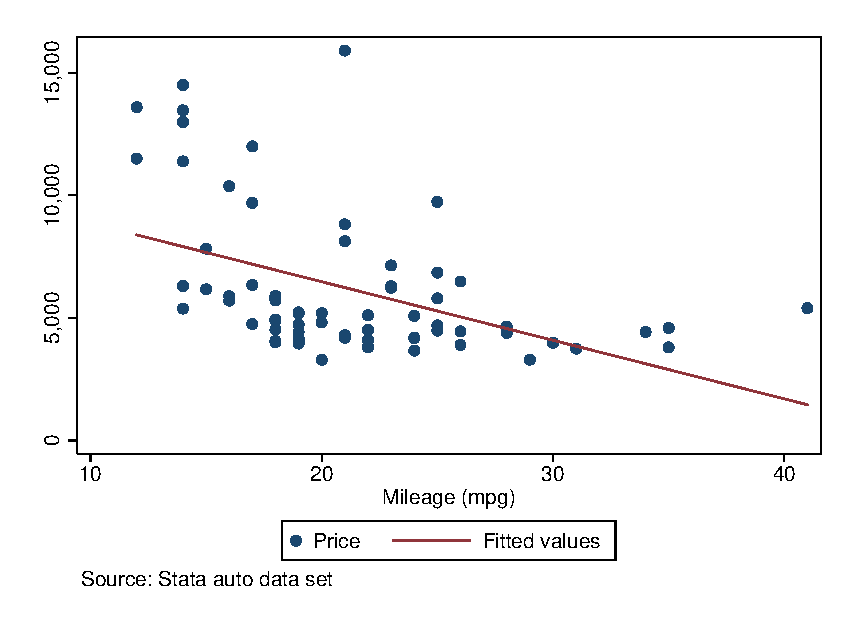
\includegraphics[width=.95\textwidth]{\results/price_mpg_figure.eps}
\end{figure}
    \end{verbatim}
    }
\end{frame}

\begin{frame}{Figure}
    \begin{figure}
        \caption{Price v. MPG}
        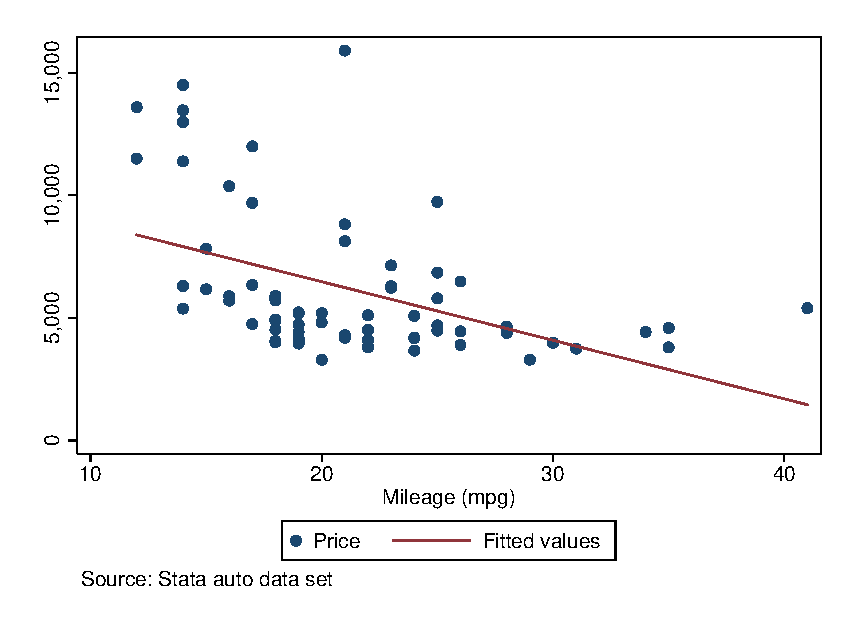
\includegraphics[width=.95\textwidth]{\results/price_mpg_figure.eps}
    \end{figure}
\end{frame}

\begin{frame}{Creating figures in Stata}
    Stata's graphics capabilities are quite powerful, although the learning curve can be somewhat steep, as there many different types of graphs and each
    type comes with a vast assortment of options. In general I recommend using do-files rather than the Stata GUI, however you may
    want to create a graph but not know the specific options you need to specify in order to add titles and axis labels, format the legend, or change
    colors. In this case simply use the Stata graphics editor to create the graph. It will then give you the code necessary to re-create the graph in both

\end{frame}

\begin{frame}{Graphics editor}
    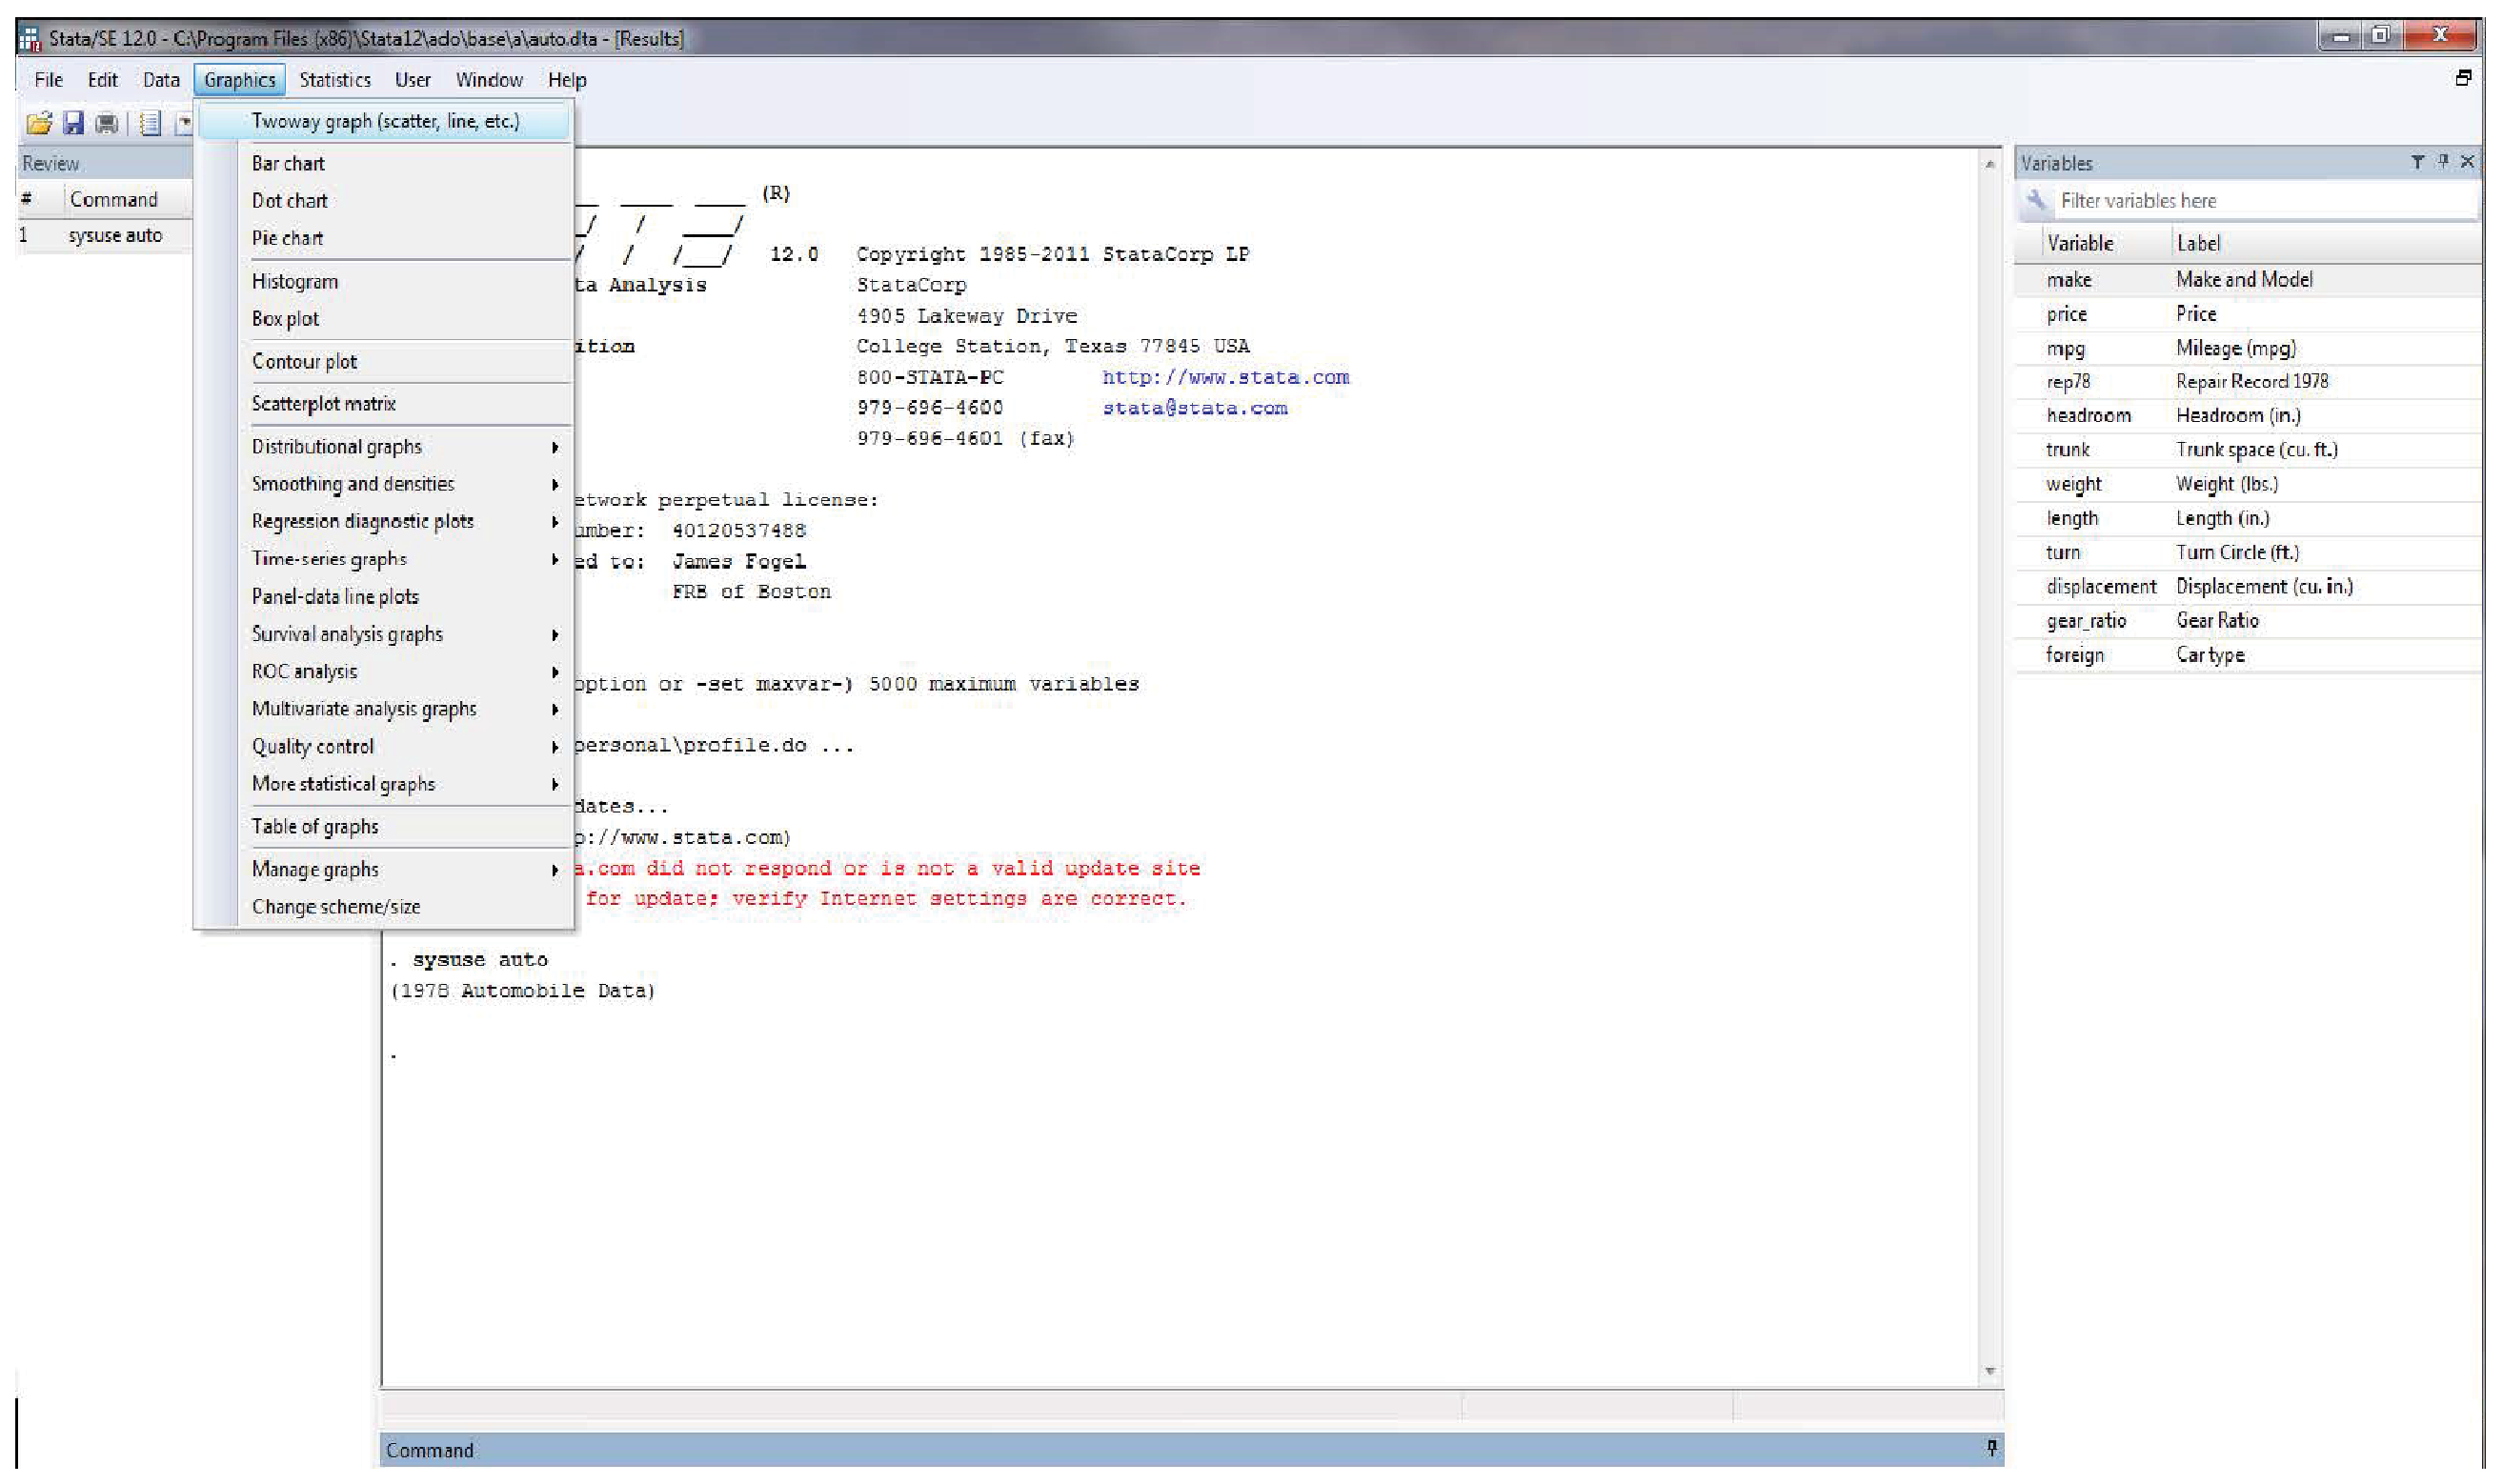
\includegraphics[width=.95\textwidth]{\results/graphics_dropdown.eps}
\end{frame}

\begin{frame}{Graphics editor}
    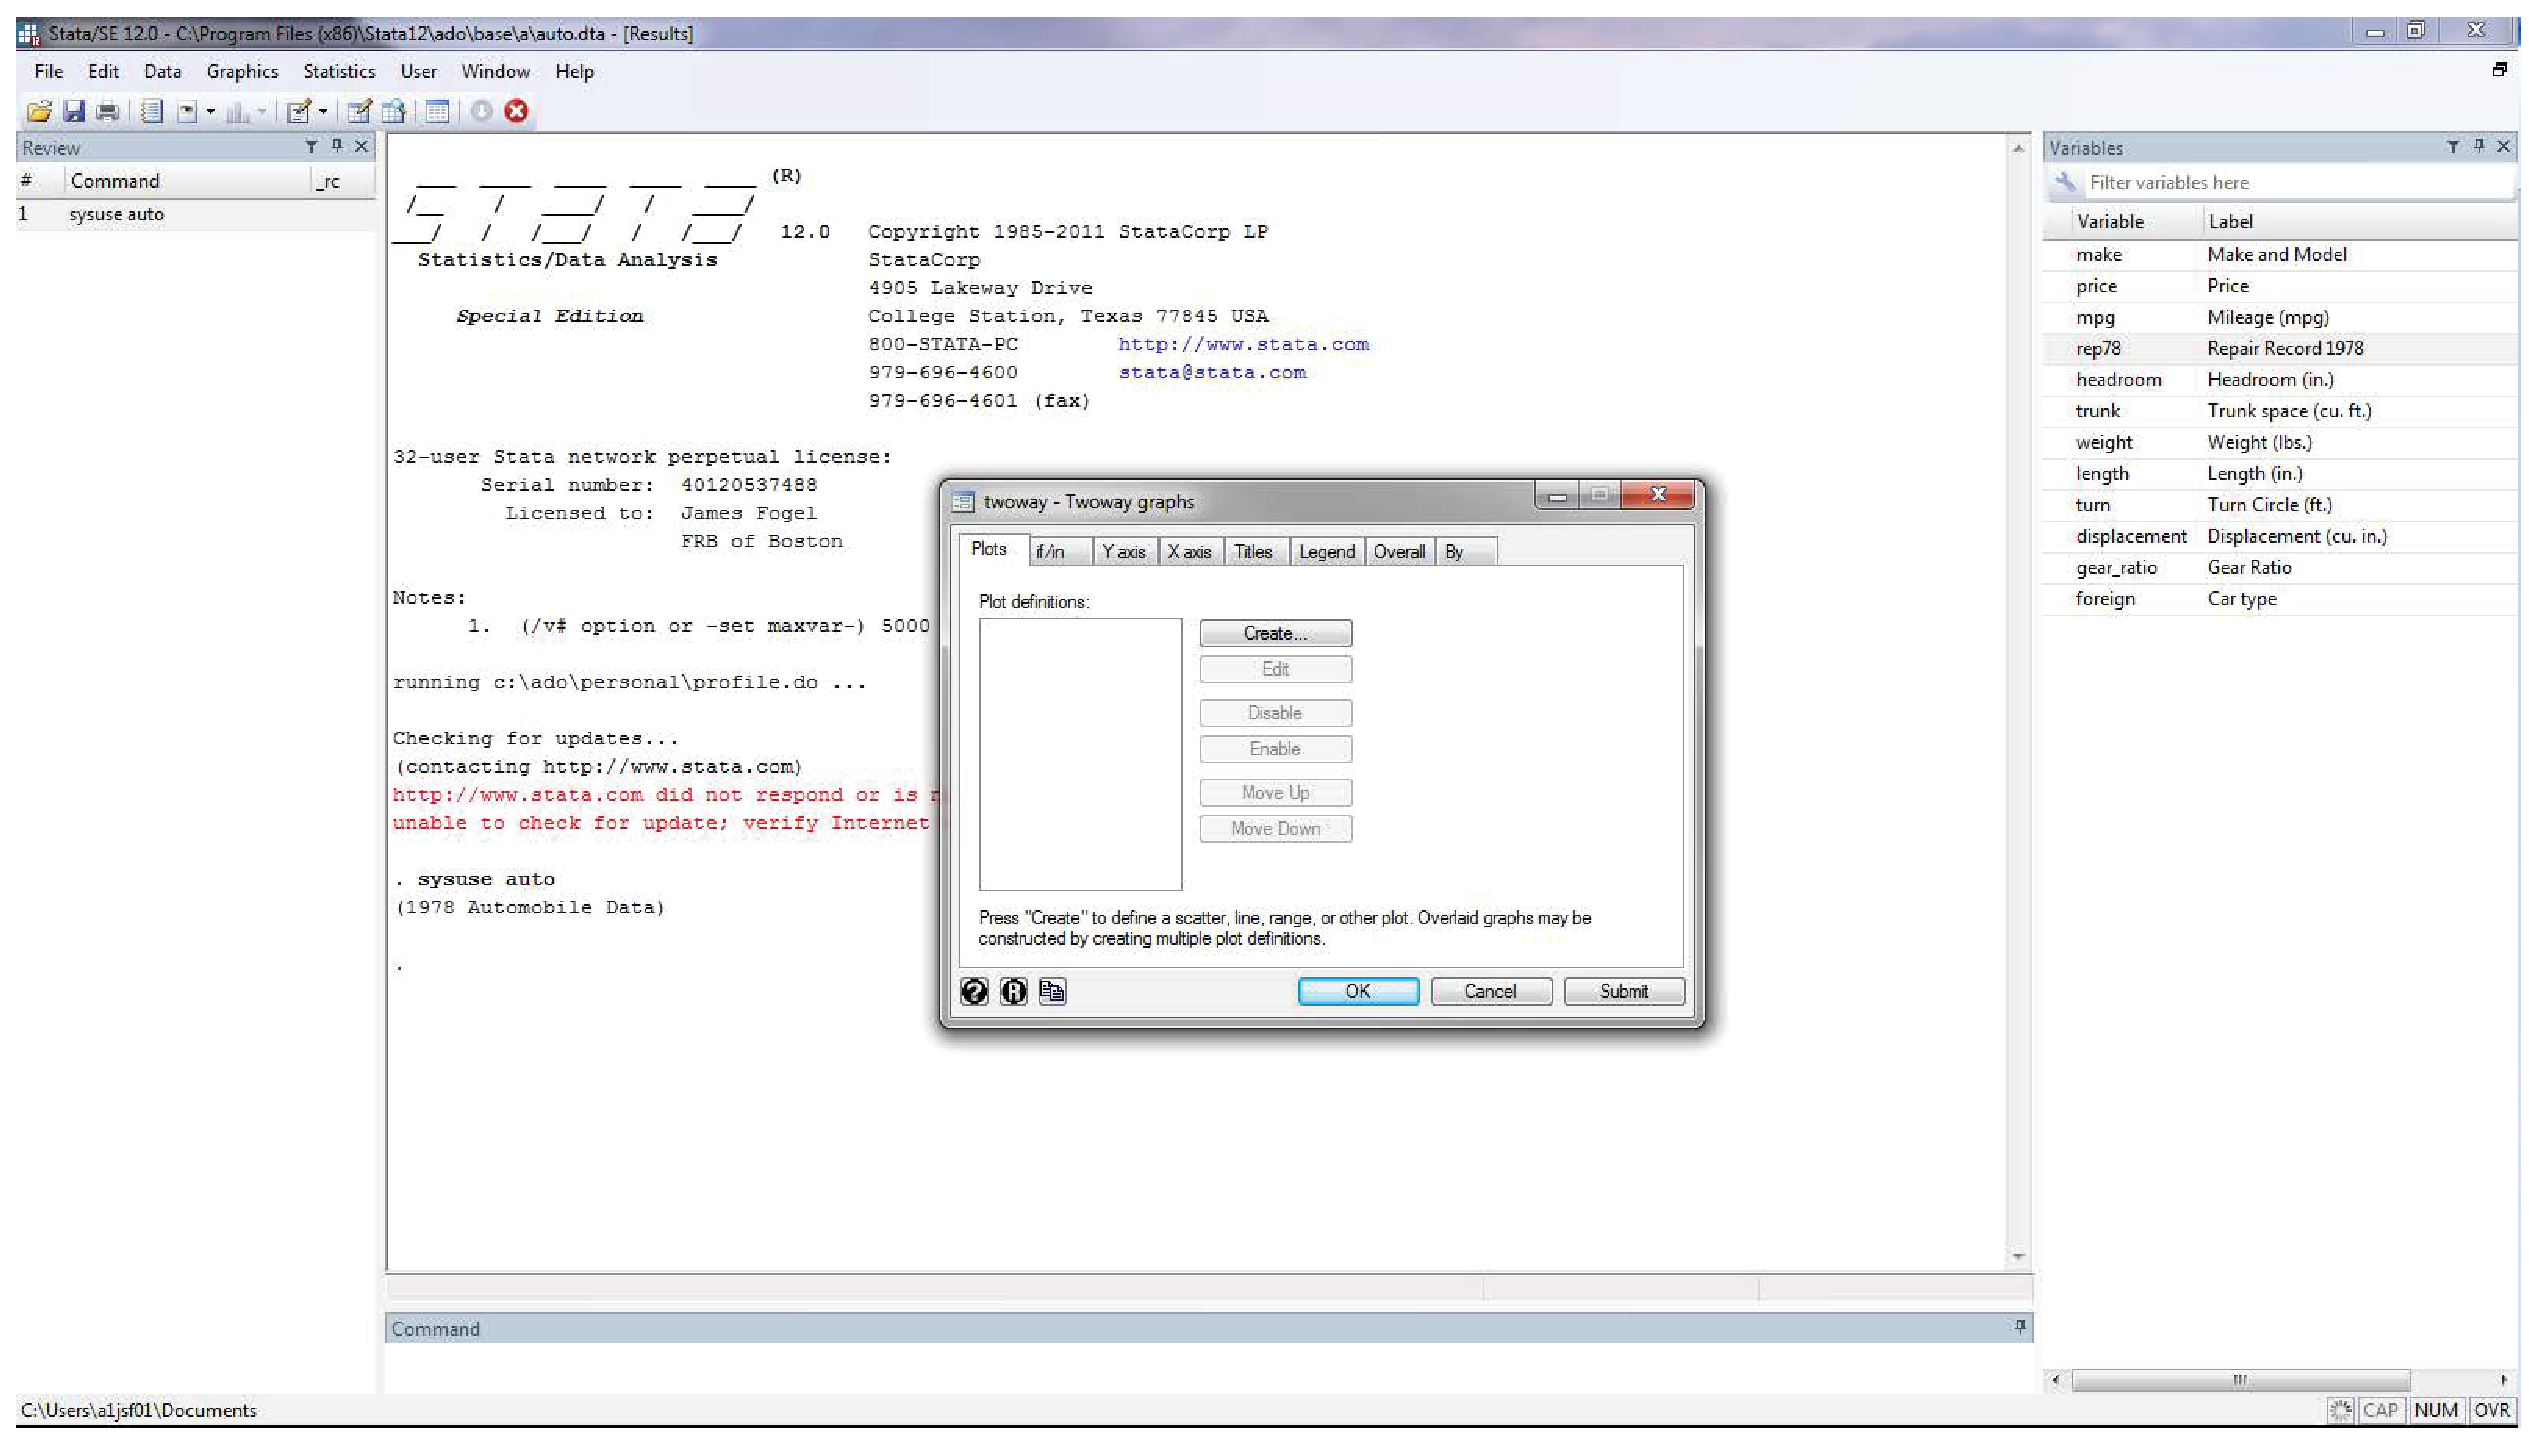
\includegraphics[width=.95\textwidth]{\results/graphics_editor.eps}
\end{frame}

\begin{frame}{Graphics editor}
    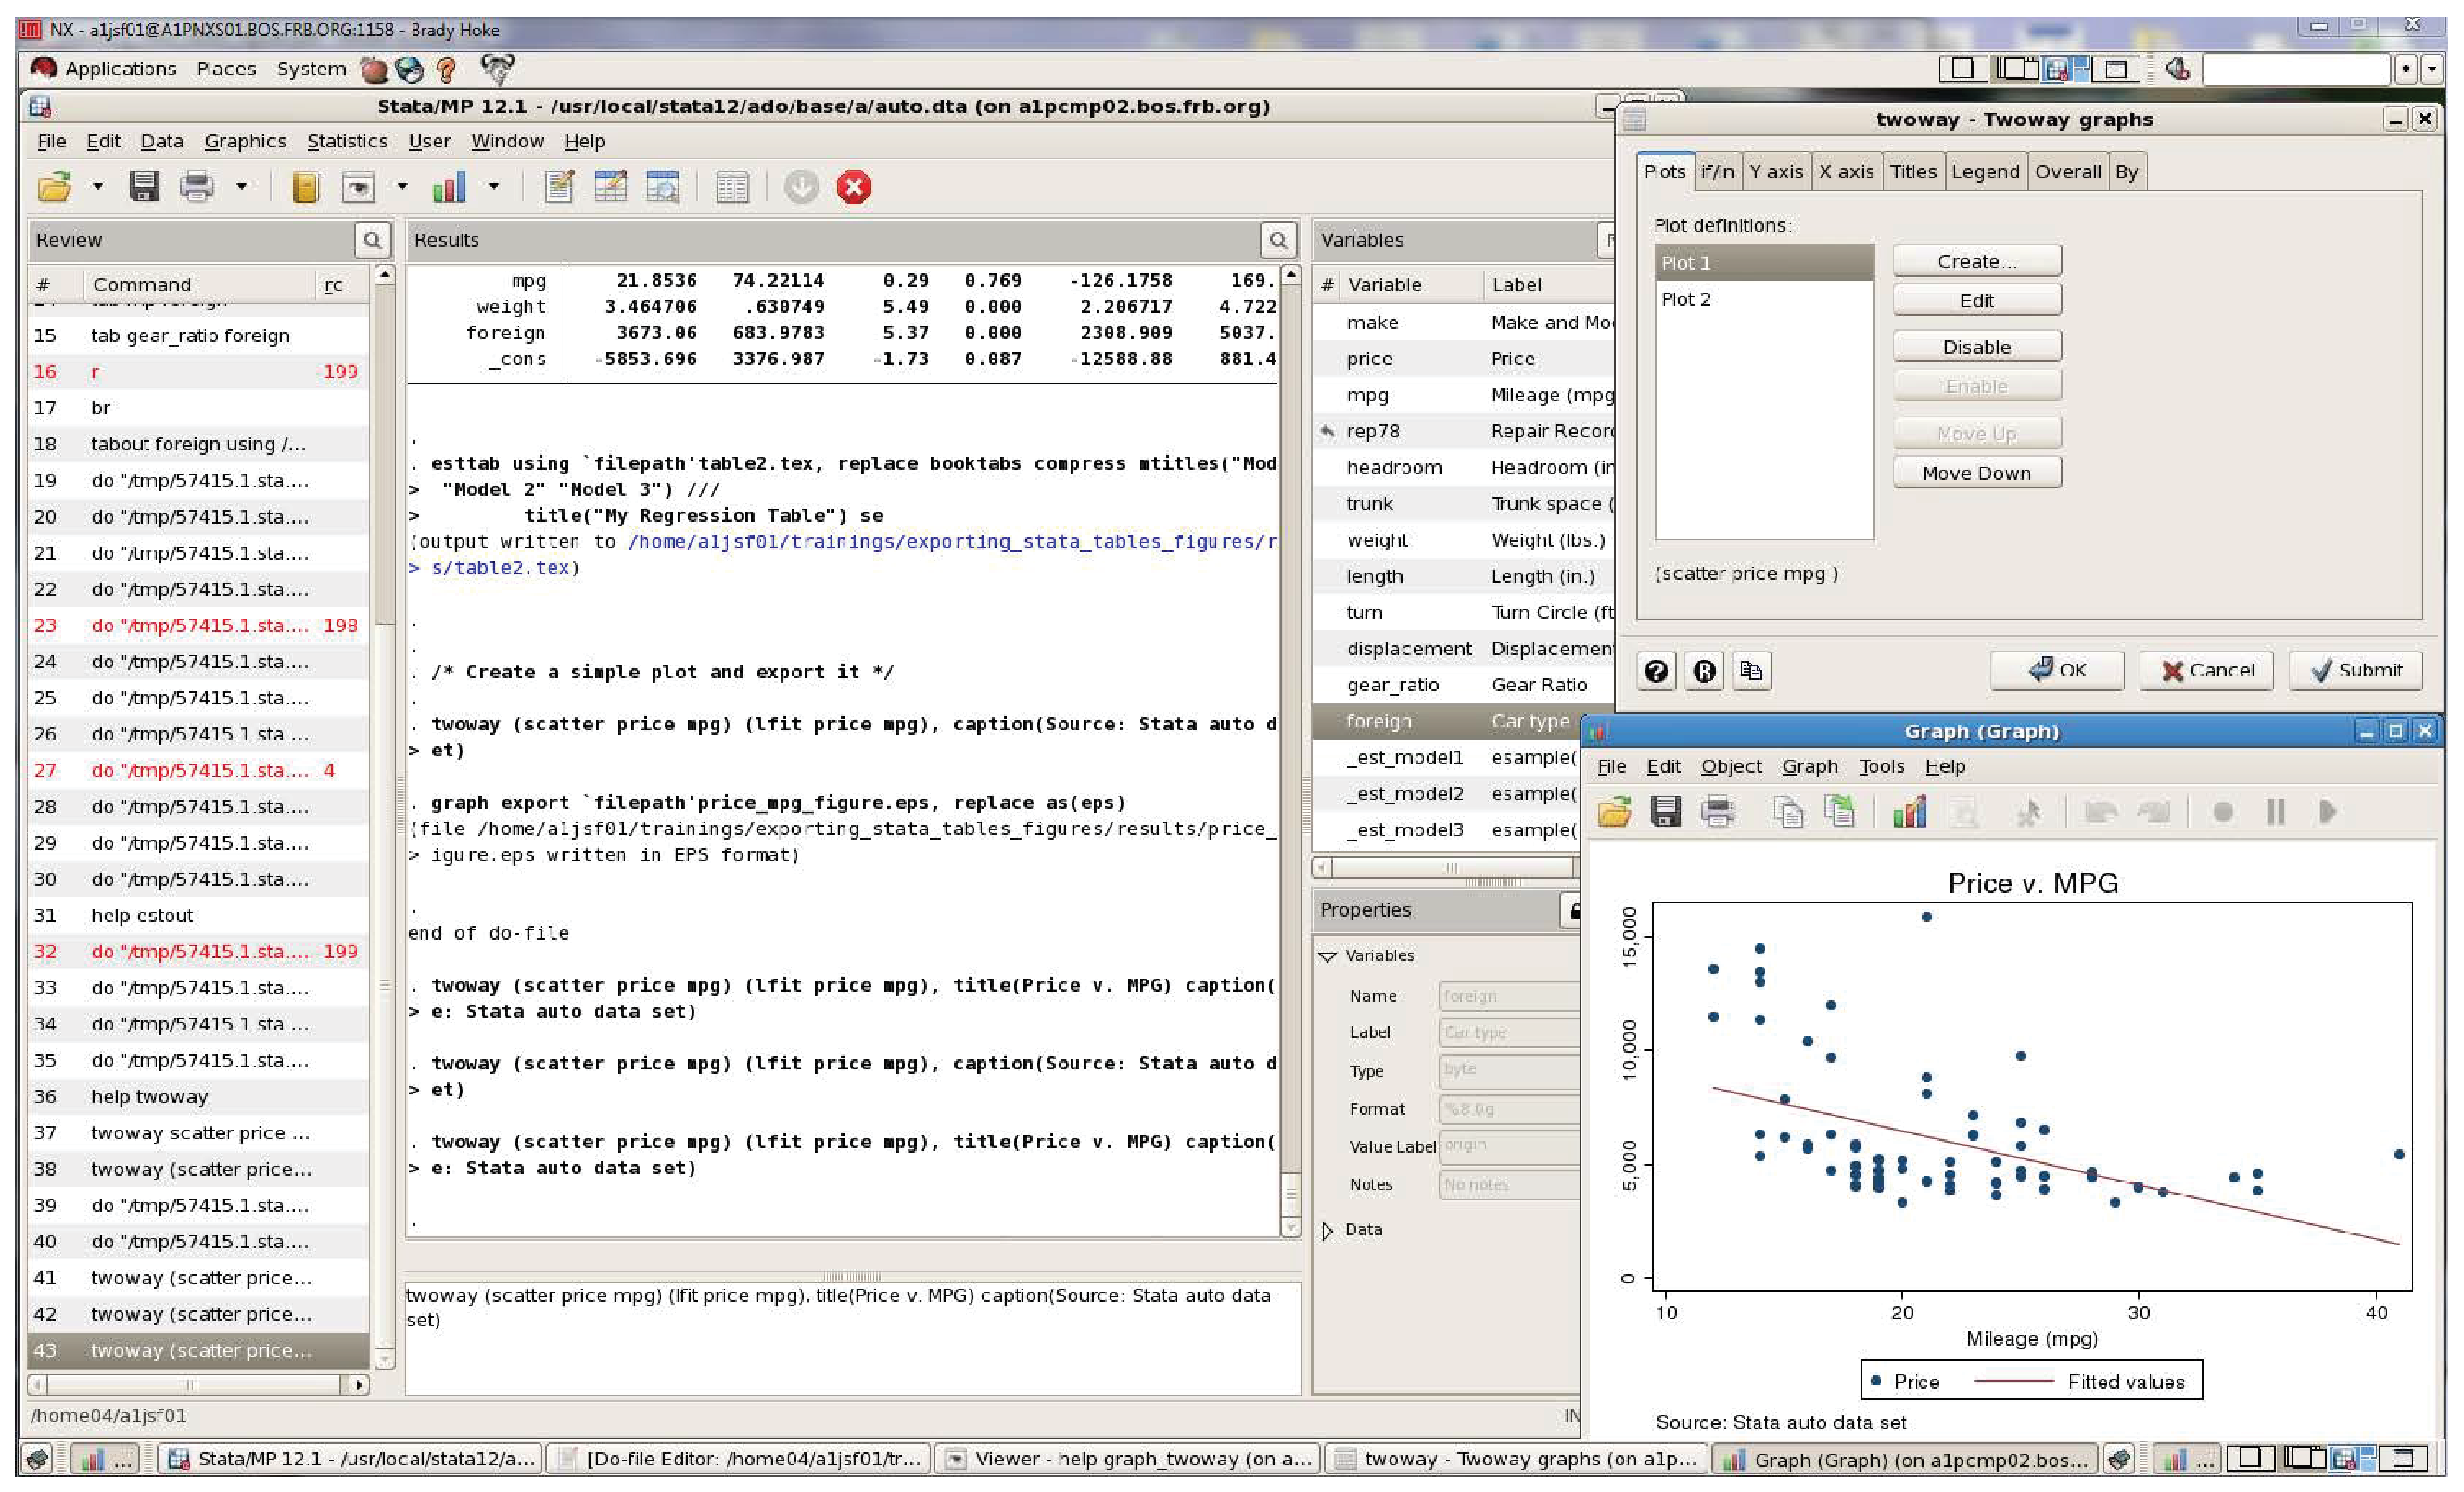
\includegraphics[width=.95\textwidth]{\results/graphics_results.eps}
\end{frame}

\section{Conclusion}

\begin{frame}{Conclusion}
    \begin{itemize}
        \item Never copy tables from Stata's result's window! Use \textbf{esttab} or \textbf{tabout} instead! \pause
        \item Once you have created a figure, it is easy to export using \textbf{graph export} \pause
        \item \LaTeX{} provides a convenient place to organize your tables and figures because making changes to tables and figures is as simple as editing your do-file,
            re-running your Stata code, and then re-compiling your \LaTeX{} document. There is NO copying and pasting and there are fewer places to make mistakes. \pause
        \item Once you have created a few tables in \textbf{tabout} or \textbf{esttab} and written a few \LaTeX{} documents you have a template for future tables and documents.
    \end{itemize}
\end{frame}


\end{document}
